\section{Actor basics}
\begin{frame}
\frametitle{Brief history of ``A Model of Concurrent Computation in Distributed Systems``}
REWORK
\begin{itemize}
\item Controversy: unbounded nondeterminism (unbounded delay yet guarantee of service)
\item Many (actively) supported languages
\item History: C. Hewitt et al. '73 \textrightarrow{} W. Clinger '81 \textrightarrow{} G. Agha '85, MIT Message Passing Semantics Group, Caltech, etc.
\item Little use around millennium, recent resurgence due to strong relevance to distributed/cloud computing (e.g. Twitter systems scalability)
\end{itemize}
\end{frame}

\begin{frame}
\frametitle{``A Model of Concurrent Computation in Distributed Systems``}
REWORK
\begin{itemize}
\item paradigm: "everything" is an actor (thread, process, core, socket, node, system, ...) \textrightarrow{} one actor encapsulates one computation unit
\item an actor may send messages to actors it knows by name
\item an (idling) actor receiving a message will accept it and execute the computation defined within, resulting in the possible actions:
	\begin{itemize}
	\item sending new messages
	\item creating new actors
	\item updating its local state
	\end{itemize}
\item an actor can only influence its own local state
\end{itemize}
\end{frame}

\begin{frame}
\frametitle{Example structure}
	\includegraphics[width=0.9\textwidth]{actorsExample}
\end{frame}

\begin{frame}
\frametitle{Hello ...}
Listing sample code
\end{frame}

\begin{frame}
\frametitle{... World!}
Output of sample code
\end{frame}